\input ../preamble

\begin{document}

{\Huge

  \centerline{\bf TTIC 31230, Fundamentals of Deep Learning}
  \bigskip
  \centerline{David McAllester, Winter 2018}
  \vfill
  \centerline{\bf Variational Autoencoders}
  \vfill
  \vfill


%these slides need more detail.  Every slide should be at least doubled.
% it also needs more material.  A theorem on noise in latent variables would be nice.



\slide{The Latent Variable Cross-Entropy Objective}

We will now drop the negation and switch to argmax.

\vfill
$${\color{red} \Phi^* = \argmax_\Phi \;\;E_{y \sim \mathrm{Pop}}  \ln Q_\Phi(y)}$$

\vfill
$${\color{red}Q_\Phi(y) = \sum_{\hat{z}} \; Q_\Phi(\hat{z},y)}$$

\vfill
EG Identity: \hspace{1em} ${\color{red} \nabla_\Phi \ln Q_\Phi(y) = \expectsub{\hat{z} \sim Q_\Phi(\hat{z}|y)}{\nabla_\Phi \;\ln Q_\Phi(\hat{z},y)}}$

\anaslide{Variational Autoencoders}
\bigskip
$${\color{red} \nabla_\Phi \ln Q_\Phi(y) = \expectsub{\hat{z} \sim Q_\Phi(\hat{z}|y)}{\nabla_\Phi \;\ln Q_\Phi(\hat{z},y)}}$$

\vfill
Except for directed tree models, this gradient must be approximated --- exact computation is \#-P hard.

\vfill
Variational autoencoders approximate $Q_\Phi(\hat{z}|y)$ with a model supporting easy sampling of $\hat{z}$.

\slide{Generative Models}

A model for which sampling is easy will be called {\bf generative}.

\vfill
In Variational autoencoders we assume that $Q_\Phi(y|\hat{z})$ is generative but that $Q_\Phi(\hat{z}|y)$ is not --- that sampling from
$Q_\Phi(\hat{z}|y)$ is hard.

\vfill
We approximate $Q_\Phi(\hat{z}|y)$ with a generative model.

\slide{Generation Replaces Search}

``Generation replaces search'' can be viewed as a general principle of Deep leaning.

\vfill
Rather than search for a $\hat{z}$ that generates $y$ we strive to directly calculate --- to generate --- a $\hat{z}$ that generates $y$.

\vfill
``Generation replaces search'' is exemplified in current parsing architectures.

\anaslide{Variational Autoencoders}
\bigskip
$$\nabla_\Phi \ln Q_\Phi(y) = \expectsub{\hat{z} \sim Q_\Phi(\hat{z}|y)}{\nabla_\Phi \;\ln Q_\Phi(\hat{z},y)}$$
\begin{eqnarray*}
\Phi^*,\Psi^* & = & \argmax_{\Phi,\Psi}\;  E_{y \sim \pop}\;\expectsub{\hat{z} \sim {\color{red} P_\Psi(\hat{z}|y)}}{\ln Q_\Phi(\hat{z},y)} + {\color{red} H(P_\Psi(\hat{z}|y))}
\end{eqnarray*}

\vfill
Here $P_\Psi(\hat{z}|y)$ is a generative approximation of $Q_\Phi(\hat{z}|y)$.

\vfill
The quantity being optimized is called the evidence lower bound (ELBO).

\anaslide{Variational Autoencoders}
\bigskip
$$\nabla_\Phi \ln Q_\Phi(y) = \expectsub{\hat{z} \sim Q_\Phi(\hat{z}|y)}{\nabla_\Phi \;\ln Q_\Phi(\hat{z},y)}$$
\begin{eqnarray*}
\Phi^*,\Psi^* & = & \argmax_{\Phi,\Psi}\; E_{y \sim \pop}\;  \expectsub{\hat{z} \sim {\color{red} P_\Psi(\hat{z}|y)}}{\ln Q_\Phi(\hat{z},y)} + {\color{red} H( P_\Psi(\hat{z}|y))} \\
\\
& = & \argmax_{\Phi,\Psi}\;E_{y \sim \pop}\;\ln Q_\Phi(y) - {\color{red} KL(P_\Psi(\hat{z}|y),\;Q_\Phi(\hat{z}|y))}
\end{eqnarray*}

\vfill
The equivalence of the two ELBO expressions is proved below.

\vfill
The first expression supports SGD training through sampling.

\vfill
The second expression establishes that the ELBO is a lower bound on the ``evidence'' $\ln Q_\Phi(y)$ and that $P_\Psi(\hat{z}|y)$ should approximate $Q_\Phi(\hat{z}|y)$.

\slide{Derivation of Equivalence I}

\begin{eqnarray*}
  & & E_{\hat{z} \sim P_\Psi(\hat{z}|y)} \;\ln Q_\Phi(\hat{z},y) \\
  \\
  & = & E_{\hat{z} \sim P_\Psi(\hat{z}|y)} \;\left(\;\ln Q_\Phi(y) + \ln Q_\Phi(\hat{z}|y)\;\right) \\
  \\
  & = & \ln Q_\Phi(y) + \;E_{\hat{z} \sim P_\Psi(\hat{z}|y)}\;\ln Q_\Phi(\hat{z}|y) \\
  \\
  & = & \ln Q_\Phi(y) - H(P_\Psi(\hat{z}|y), Q_\Phi(\hat{z}|y))
\end{eqnarray*}

\slide{Derivation of Equivalence II}
\begin{eqnarray*}
  & & \expectsub{\hat{z} \sim P_\Psi(\hat{z}|y)}{\ln Q_\Phi(\hat{z},y)} + H(P_\Psi(\hat{z}|y))\\
  \\
  & = & \ln Q_\Phi(y) - H(P_\Psi(\hat{z}|y), Q_\Phi(\hat{z}|y)) + H(P_\Psi(\hat{z}|y)) \\
  \\
  & = & \ln Q_\Phi(y) - KL(P_\Psi(\hat{z}|y),Q_\Phi(\hat{z}|y)) \\
\end{eqnarray*}

\slide{EM is Alternating Optimization of the ELBO}

\begin{eqnarray*}
& & E_{\hat{z} \sim P_\Psi(\hat{z}|y)}\; \ln Q_\Phi(\hat{z},y) + H(P_\Psi(\hat{z}|y))\;\;\;(1) \\
 \\      
  & = & \ln\;Q_{\Phi}(y) - KL(P_\Psi(\hat{z}|y),Q_{\Phi}(\hat{z}|y))\;\;\;\;\;\;(2)
\end{eqnarray*}

\vfill
$$\mbox{by (2)}\;\;\;\Psi^* = \argmin_\Psi E_{y \sim \pop} \; KL(P_\Psi(\hat{z}|y),Q_\Phi(\hat{z}|y))$$

$$\mbox{by (1)}\;\;\;\Phi^* = \argmax_\Phi E_{y \sim \pop} \;E_{\hat{z} \sim P_\Psi(\hat{z}|y)}\; \ln Q_\Phi(\hat{z},y)$$

\vfill
EM: $\Phi^{\color{red} t+1} = \argmax_{\color{red} \Phi} \; E_{y \sim \pop}\; E_{\hat{z} \sim Q_{\Phi^{\color{red} t}}(\hat{z}|y)}\; \;\log Q_{\color{red} \Phi}(\hat{z},y)$

\vfill
\anaslide{The Reparameterization Trick}
\bigskip
\begin{eqnarray*}
\Psi^* & = & \argmax_\Psi \; E_{y \sim \pop}\;\expectsub{\color{red} \hat{z} \sim P_\Psi(\hat{z}|y)}{\ln Q_\Phi(\hat{z},y)} + H(P_\Psi(\hat{z}|y))
\end{eqnarray*}

\vfill
How do we differentiate the sampling?

\vfill
\anaslide{The Reparameterization Trick}
\bigskip
\begin{eqnarray*}
\Psi^* & = & \argmax_\Psi \; E_{y \sim \pop}\;\expectsub{\color{red} \hat{z} \sim P_\Psi(\hat{z}|y)}{\ln Q_\Phi(\hat{z},y)} + H(P_\Psi(\hat{z}|y))
\end{eqnarray*}

\vfill
We note that in practice all sampling is computed by a deterministic function of (pseudo) random numbers.

\vfill
We can make this explicit.

\vfill
Model $P_\Psi(\hat{z}|y)$ by $\epsilon \sim \mathrm{noise}$, $\hat{z} = \hat{z}_\Psi(y,\epsilon)$

\vfill
\anaslide{The Reparameterization Trick}
\bigskip
\begin{eqnarray*}
\Psi^* & = & \argmax_\Psi \; E_{y \sim \pop}\;\expectsub{\color{red} \epsilon \sim \mathrm{noise}}{\ln Q_\Phi({\color{red} \hat{z}_\Psi(y,\epsilon)},y)} +  H(P_\Psi(\hat{z}|y)) \\
\\
H(P_\Psi(\hat{z}|y)) & = & \expectsub{\color{red} \epsilon \sim \mathrm{noise}} {\ln P_\Psi({\color{red} \hat{z}_\Psi(y,\epsilon)}|y)}
\end{eqnarray*}

\vfill
For VAEs we typically we have $\hat{z}(y,\epsilon) \in \mathbb{R}^d$ with
\begin{eqnarray*}
\hat{z}(y,\epsilon)[i] & = & \mu_\Psi(y)[i] + \sigma_\Psi(y)[i]\;\epsilon[i] \\
\epsilon[i] & \sim & {\cal N}(0,1)
\end{eqnarray*}

\vfill
This supports easy calculation of $P_\Psi(\hat{z}_\Psi(y,\epsilon)|y)$.

\slide{Decoding with $L_2$ Distortion}

An autoencoder {\bf encodes} and {\bf decodes}.

\vfill
We can view $\hat{z}_\Psi(y,\epsilon)$ as the encoding of $y$.

\vfill
We now consider a deterministic decoder $\hat{y}_\Phi(\hat{z})$ and define a model

$${\color{red} Q_\Phi(y|\hat{z}) \propto \exp\left(\frac{- ||y - \hat{y}_\Phi(\hat{z})||^2}{2\sigma^2}\right)}$$

\slideplain{A VAE for Images}

Auto-Encoding Variational Bayes, Diederik P Kingma, Max Welling, 2013.

\vfill
$${\color{red}y \hspace{5em}  \hat{z}_\Psi(y,\epsilon) \hspace{4em} \hat{z} \hspace{6em} \hat{y}_\Phi(\hat{z}) \hspace{4em}||y - \hat{y}||^2}$$
\centerline{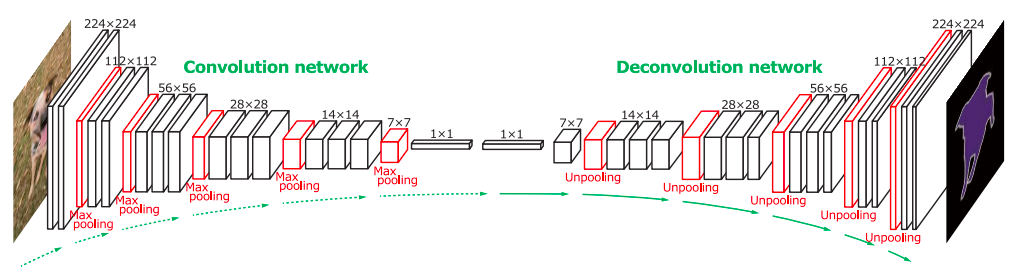
\includegraphics[width=9in]{../images/Deconv}}

\centerline{\Large [Hyeonwoo Noh et al.]}



\slide{Deconvoution: Increasing Spatial Dimension}

Consider a stride 2 convolution
\begin{eqnarray*}
  y[i,j,c_y] & = &   W[\Delta i, \Delta j, c_x, c_y] x[2i + \Delta i, 2j + \Delta j, c_x] \\
  y[i,j,c_y] & \pluseq & B[c_y]
\end{eqnarray*}

\vfill
For deconvolution we use stride 1 with 4 times the channels.
\begin{eqnarray*}
  \hat{x}[i,j,c_{\hat{x}}] & = &   W'[\Delta i, \Delta j, c_{\hat{y}}, c_{\hat{x}}] \hat{y}[i + \Delta i, j + \Delta j, c_{\hat{x}}] \\
  \hat{x}[i,j,c_{\hat{x}}] & \pluseq & B[c_{\hat{x}}]
\end{eqnarray*}

\vfill
The channels at each lower resolution pixel $\hat{x}[i,j]$ are divided among four higher resolution pixels.

\vfill
This is done by a simple reshaping of $\hat{x}$.

\slide{Decoding with $L_2$ Distortion}

\begin{eqnarray*}
\Phi^*,\Psi^* & = & \argmax_{\Phi,\Psi}\; E_{y \sim \pop}\; \expectsub{\hat{z} \sim P_\Psi(\hat{z}|y)}{\ln Q_\Phi(\hat{z},y)} + H(P_\Psi(\hat{z}|y))
\end{eqnarray*}

\vfill
The objective now becomes

\vfill
$$E_{y \sim \pop}\;\expectsub{\hat{z}\sim P_\Psi(\hat{z}|y)} \left(\ln P_\Phi(\hat{z}) - \frac{1}{2\sigma^2}\left|\left|y - \hat{y}_\Phi(\hat{z})\right|\right|^2\right) + H(P_\Psi(\hat{z}|y))$$

\slide{Decoding with $L_2$ Distortion}

Switching back to minimization, we can now rewrite the objective as

\vfill
$$\min \; \expectsub{y,\epsilon} \;\left(|\hat{z}_\Psi(y,\epsilon)|_\Phi +  \frac{1}{2}\lambda||y - \hat{y}_\Phi(\hat{z}_\Psi(y,\epsilon))||^2\right) - |\hat{z}_\Psi(y,\epsilon)|_{\Psi,y}$$

\vfill
$$|\hat{z}|_\Phi  = - \log_2 P_\Phi(\hat{z})\hspace{5em} |\hat{z}|_{\Psi,y}  = - \log_2 P_\Psi(\hat{z}|y)$$

\vfill
For $\hat{z}$ discrete, $|\hat{z}|_\Phi$ is the code length of $\hat{z}(y,\epsilon)$ under an optimal code for $P_\Phi$.

\vfill
$|\hat{z}|_{\Psi,y}$ is the code length for $\hat{z}$ under the code for $P_\Psi(\hat{z}|y)$.

\slide{Soft EM is to Hard EM as VAE is to Rate-Distortion}

(Soft) EM: $\Phi^{\color{red} t+1} = \argmax_{\color{red} \Phi} E_{y \sim \pop}\;\;\;E_{\hat{z} \sim Q_{\Phi^{\color{red} t}}(\hat{z}|y)}\; \;\log Q_{\color{red} \Phi}(\hat{z},y)$

\vfill
Hard EM: $\Phi^{\color{red} t+1} = \argmax_{\color{red} \Phi}\; E_{y \sim \pop}\;Q_{\color{red} \Phi}(\hat{z}(y),y)$
$$\hspace{17em} \hat{z}(y) = \argmax_{\hat{z}}\;Q_{\Phi^{\color{red} t}}(\hat{z}|y)$$

\vfill
VAE: $\min \expectsub{y,\epsilon} |\hat{z}_\Psi(y,\epsilon)|_\Phi +  \frac{1}{2}\lambda||y - \hat{y}_\Phi(\hat{z}_\Psi(y,\epsilon))||^2 - |\hat{z}_\Psi(y,\epsilon)|_{\Psi,y}$

\vfill
RD:  $\min \expectsub{y} |\hat{z}_\Psi(y)|_\Phi +  \frac{1}{2}\lambda||y - \hat{y}_\Phi(\hat{z}_\Psi(y))||^2$



\slideplain{Sampling}

$$P_\Psi(\hat{z}|y) \hspace{3ex} \hat{z} \hspace{3ex}  Q_\Phi(\hat{z},y)$$

\centerline{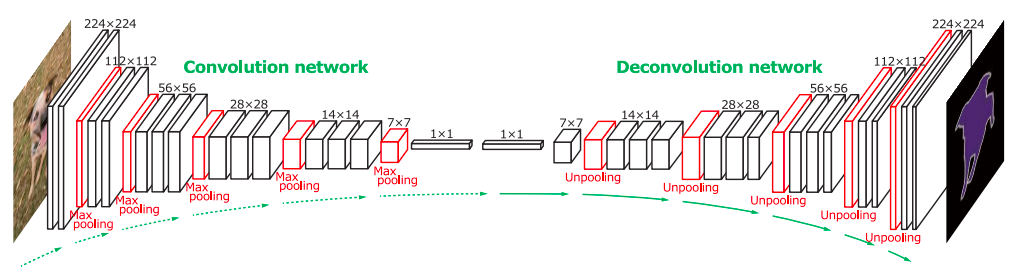
\includegraphics[width=6in]{../images/Deconv}}
\centerline{\large [Hyeonwoo Noh et al.]}

\vfill
Sampling uses just the second half ${\color{red} Q_\Phi(\hat{z},y)}$.

\slide{Sampling from Gaussian Variational Autoencoders}

\vfill
\centerline{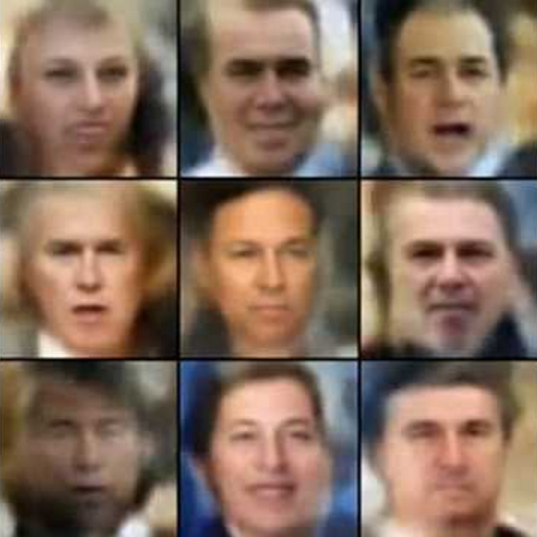
\includegraphics[width = 4in]{../images/VariationalFaces}}
\centerline{[Alec Radford]}

\slide{Why Blurry?}

A common explanation for the blurryness of images generated from VAEs is the use of $L_2$ as the distortion measure.

\vfill
It does seem that $L_1$ works better (see the slides on image-to-image GANs).

\vfill
However, training on $L_2$ distortion can produce sharp images in rate-distortion autoencoders (see the slides on rate-distortion autoencoders).
\slide{END}

}
\end{document}

